\section{Studien zur Browserkompatibilität}
\label{sec:studien-zur-browser-kompatibilitaet}

Im \autoref{sec:browserprodukte} wurde die Anzahl an Studien zur Browserkompatiblität dargestellt. Dabei wurde in der Suche jeweils bei den Optionen \texttt{von} und \texttt{bis} des Erscheinungsjahres jedes Jahr einzeln eingegeben und eine Suche durchgeführt, die Trefferanzahl wurde dann notiert. Die Daten hierfür wurden über die Literatursuchmaschine \enquote{Google Scholar} am 25.02.2021 abgerufen. Für die Suche wurde folgender Suchterm benutzt:
\begin{verbatim}
"cross browser" compatibility|incompatibility|inconsistency|XBI
\end{verbatim}

\begin{wraptable}[10]{r}{0.42\linewidth}
\centering
\vspace{-\baselineskip}
\begin{tabular}{|l|l|}
  \hline
  Jahr & Suchtreffer \\
  \hline
  2015 & 272 \\
  \hline
  2016 & 228 \\
  \hline
  2017 & 208 \\
  \hline
  2018 & 204 \\
  \hline
  2019 & 172 \\
  \hline
  2020 & 167 \\
  \hline
\end{tabular}
\caption{Suchtreffer zu Studien über Browserkompatibilität}
	\label{tab:suchtreffer-metastudie}
\end{wraptable}

\def\lc{\left\lceil}   
\def\rc{\right\rceil}

Die jahresbezogene Trefferanzahl (vgl. \autoref{tab:suchtreffer-metastudie}) soll aufdecken, ob ein Trend in der Literatur zu erkennen ist. Ein schwacher, aber vorhandener Negativtrend konnte festgestellt werden.

Weiterhin lässt sich dieselbe Thematik bei Google Trends \cite{GoogleTrendsCrossBrowserCompatibility} untersuchen. Hierbei wurden die Suchtrends für den Suchterm \texttt{cross browser compatability} abgerufen und geplotted (vgl. \autoref{fig:google-search-trends_cross-browser-compatability}). Dabei lässt sich ebenso ein Negativtrend erkennen.

\begin{figure}[H]
	\centering
	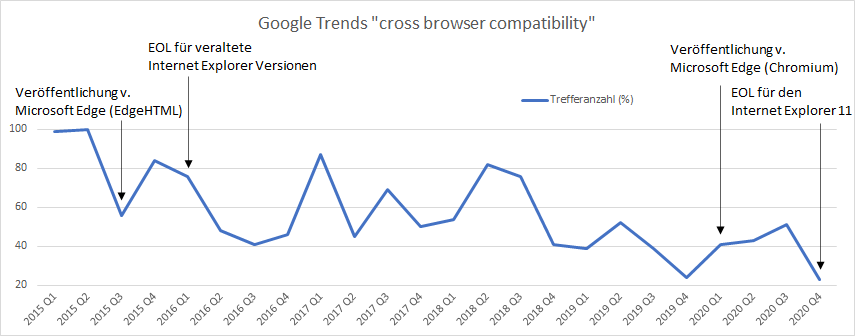
\includegraphics[width=0.84\linewidth]{img/99_postscript/google-trends_cross-browser-compatability.png}
	\caption{Google Trends zur Browserkompatibilität, angereichert mit \cite{MicrosoftIEandEdgeLifecycleFAQ}}
	\label{fig:google-search-trends_cross-browser-compatability}
\end{figure}

\section{Weitere Demonstration}
\label{sec:weitere-demonstration}

\subsection{LogRocket}
\label{sec:demo-logrocket}

Im Anhang befindet sich ein Video, welches die Aufnahme eines Session-Replays von LogRocket ist. Das eigentliche Session-Replay erfolgt interaktiv im Browser und Daten wie der DOM, die Konsole und auch Netzwerkaufrufe können vom Entwickler inspiziert werden.

\subsection{Splunk}
\label{sec:demo-splunk}

Neben Logs wurden in Splunk zudem auch Metriken und Fehler erhoben. Bei Metriken handelt es sich um beispielhafte Daten, die veranschaulichen und beweisen sollen, dass das Konzept funktioniert. Genauer wurden zwei wesentliche Metriken aufgezeichnet, einerseits die Anzahl an Produkten im Warenkorb und andererseits die aufgetretenen Fehler in einer Sitzung. Diese Metriken wurden auf einer Seite in Splunk visuell dargestellt, welche in \autoref{fig:splunk_metric-overview} zu sehen ist.

\begin{figure}[H]
	\centering
	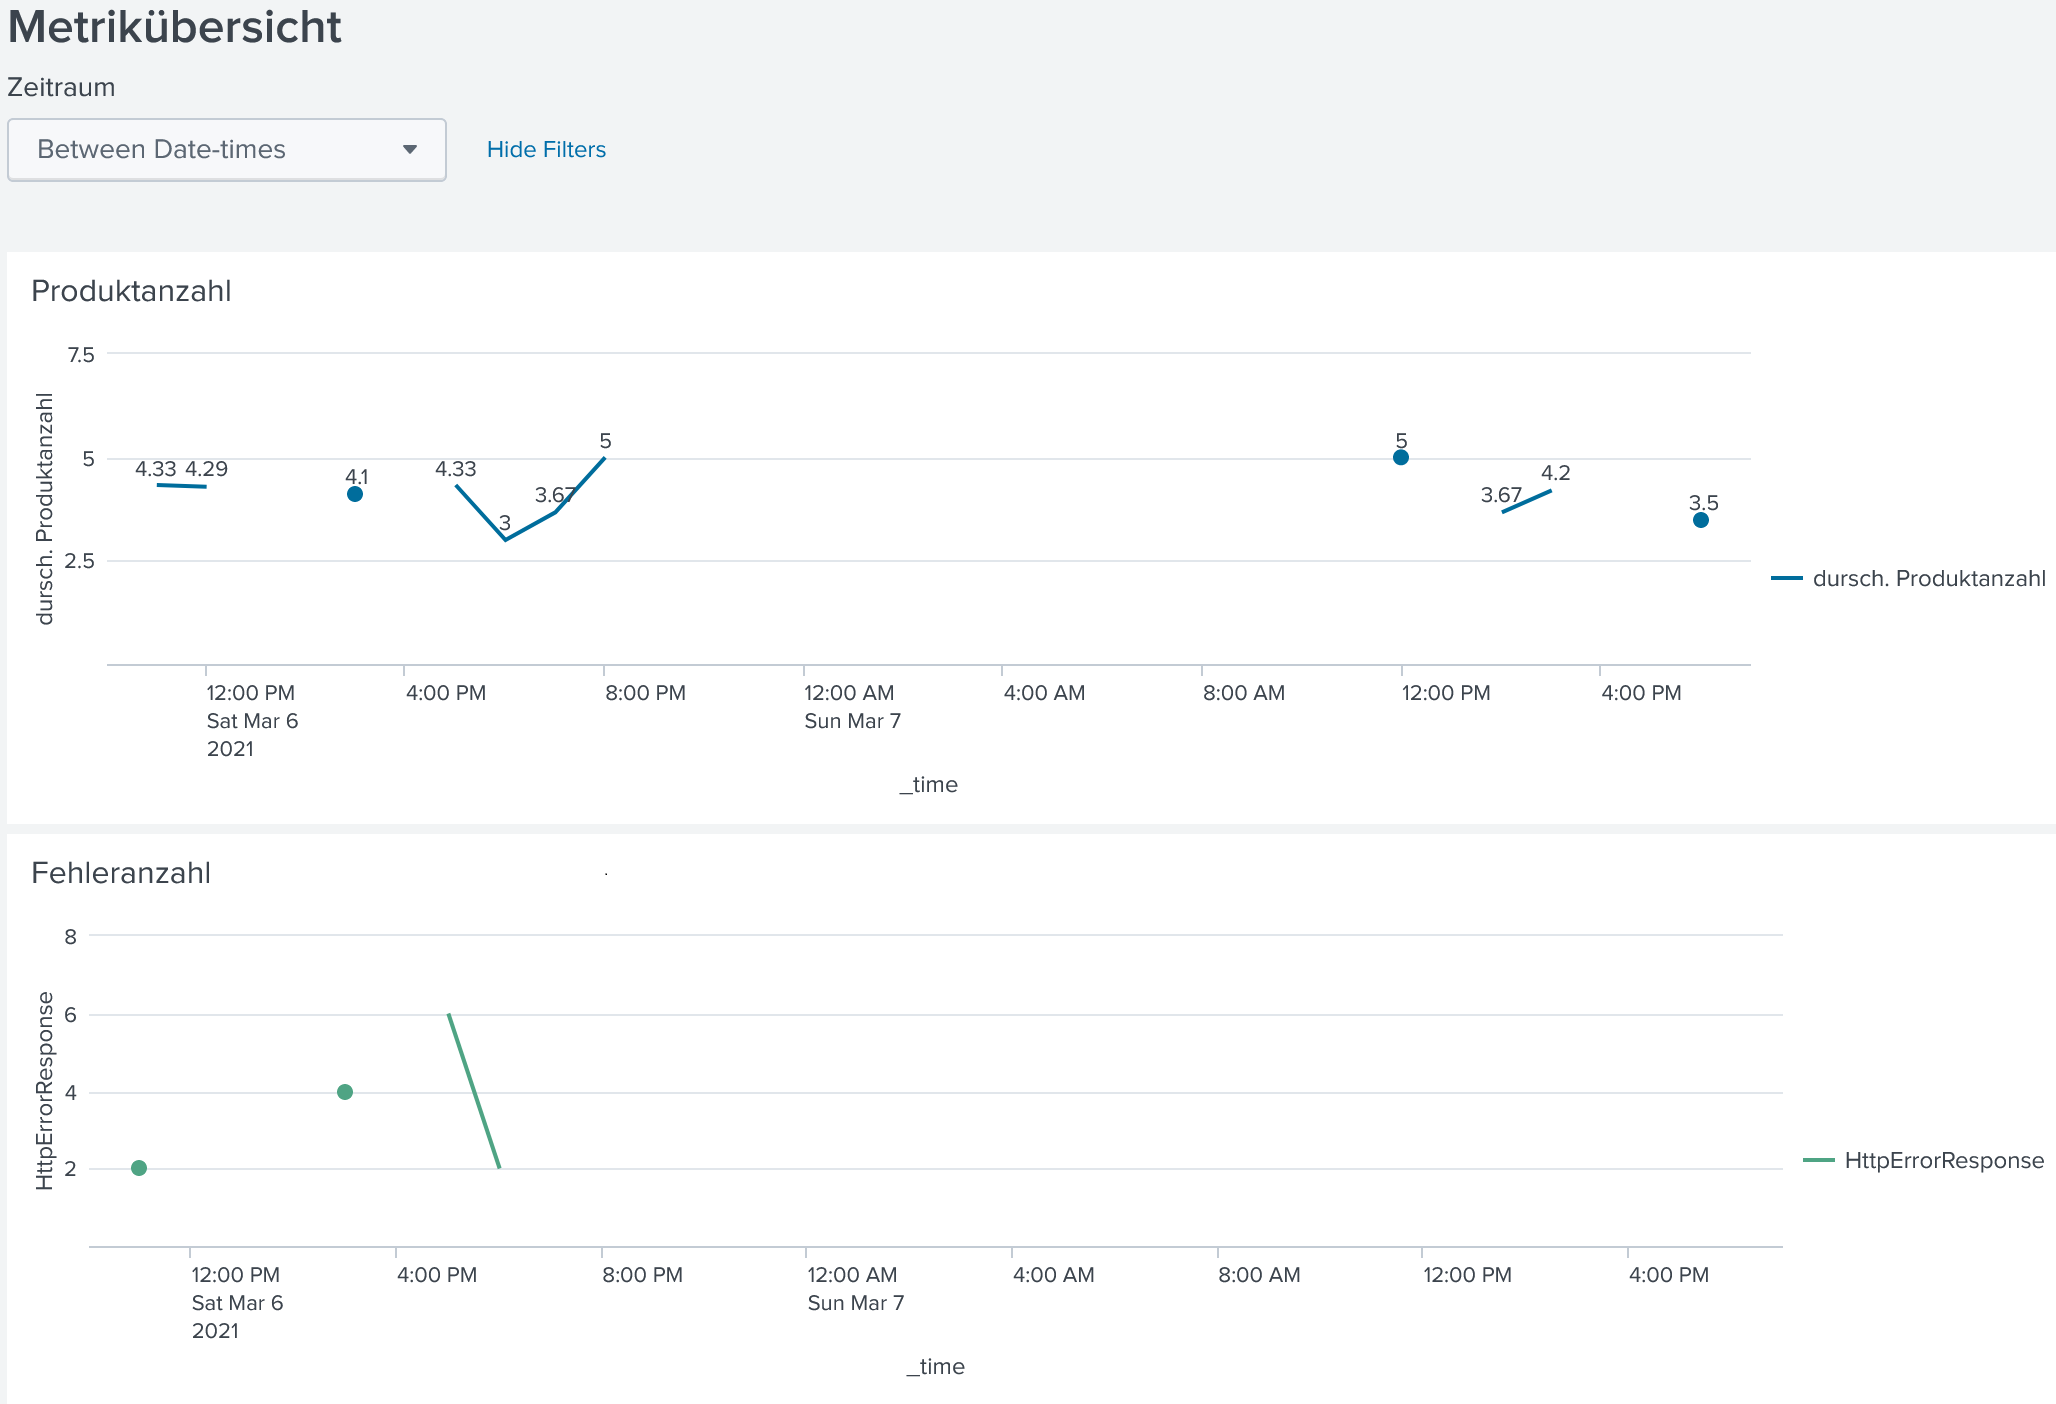
\includegraphics[width=1.00\linewidth]{img/99_postscript/splunk_metric-overview.png}
	\caption{Metrikübersicht in Splunk}
	\label{fig:splunk_metric-overview}
\end{figure}

Um speziell Fehler zu visualisieren und diese auch gruppiert darzustellen, wurde in Splunk eine Seite hierfür erstellt \autoref{fig:splunk_error-dashboard}. In der Fehlerübersicht lassen sich ein Histogramm, ein Top-Chart sowie die letzten 50 Events im Detail betrachten. Hierbei ließe sich bspw. ein erhöhtes Fehleraufkommen feststellen, das von der Norm abweicht.

\begin{figure}[H]
	\centering
	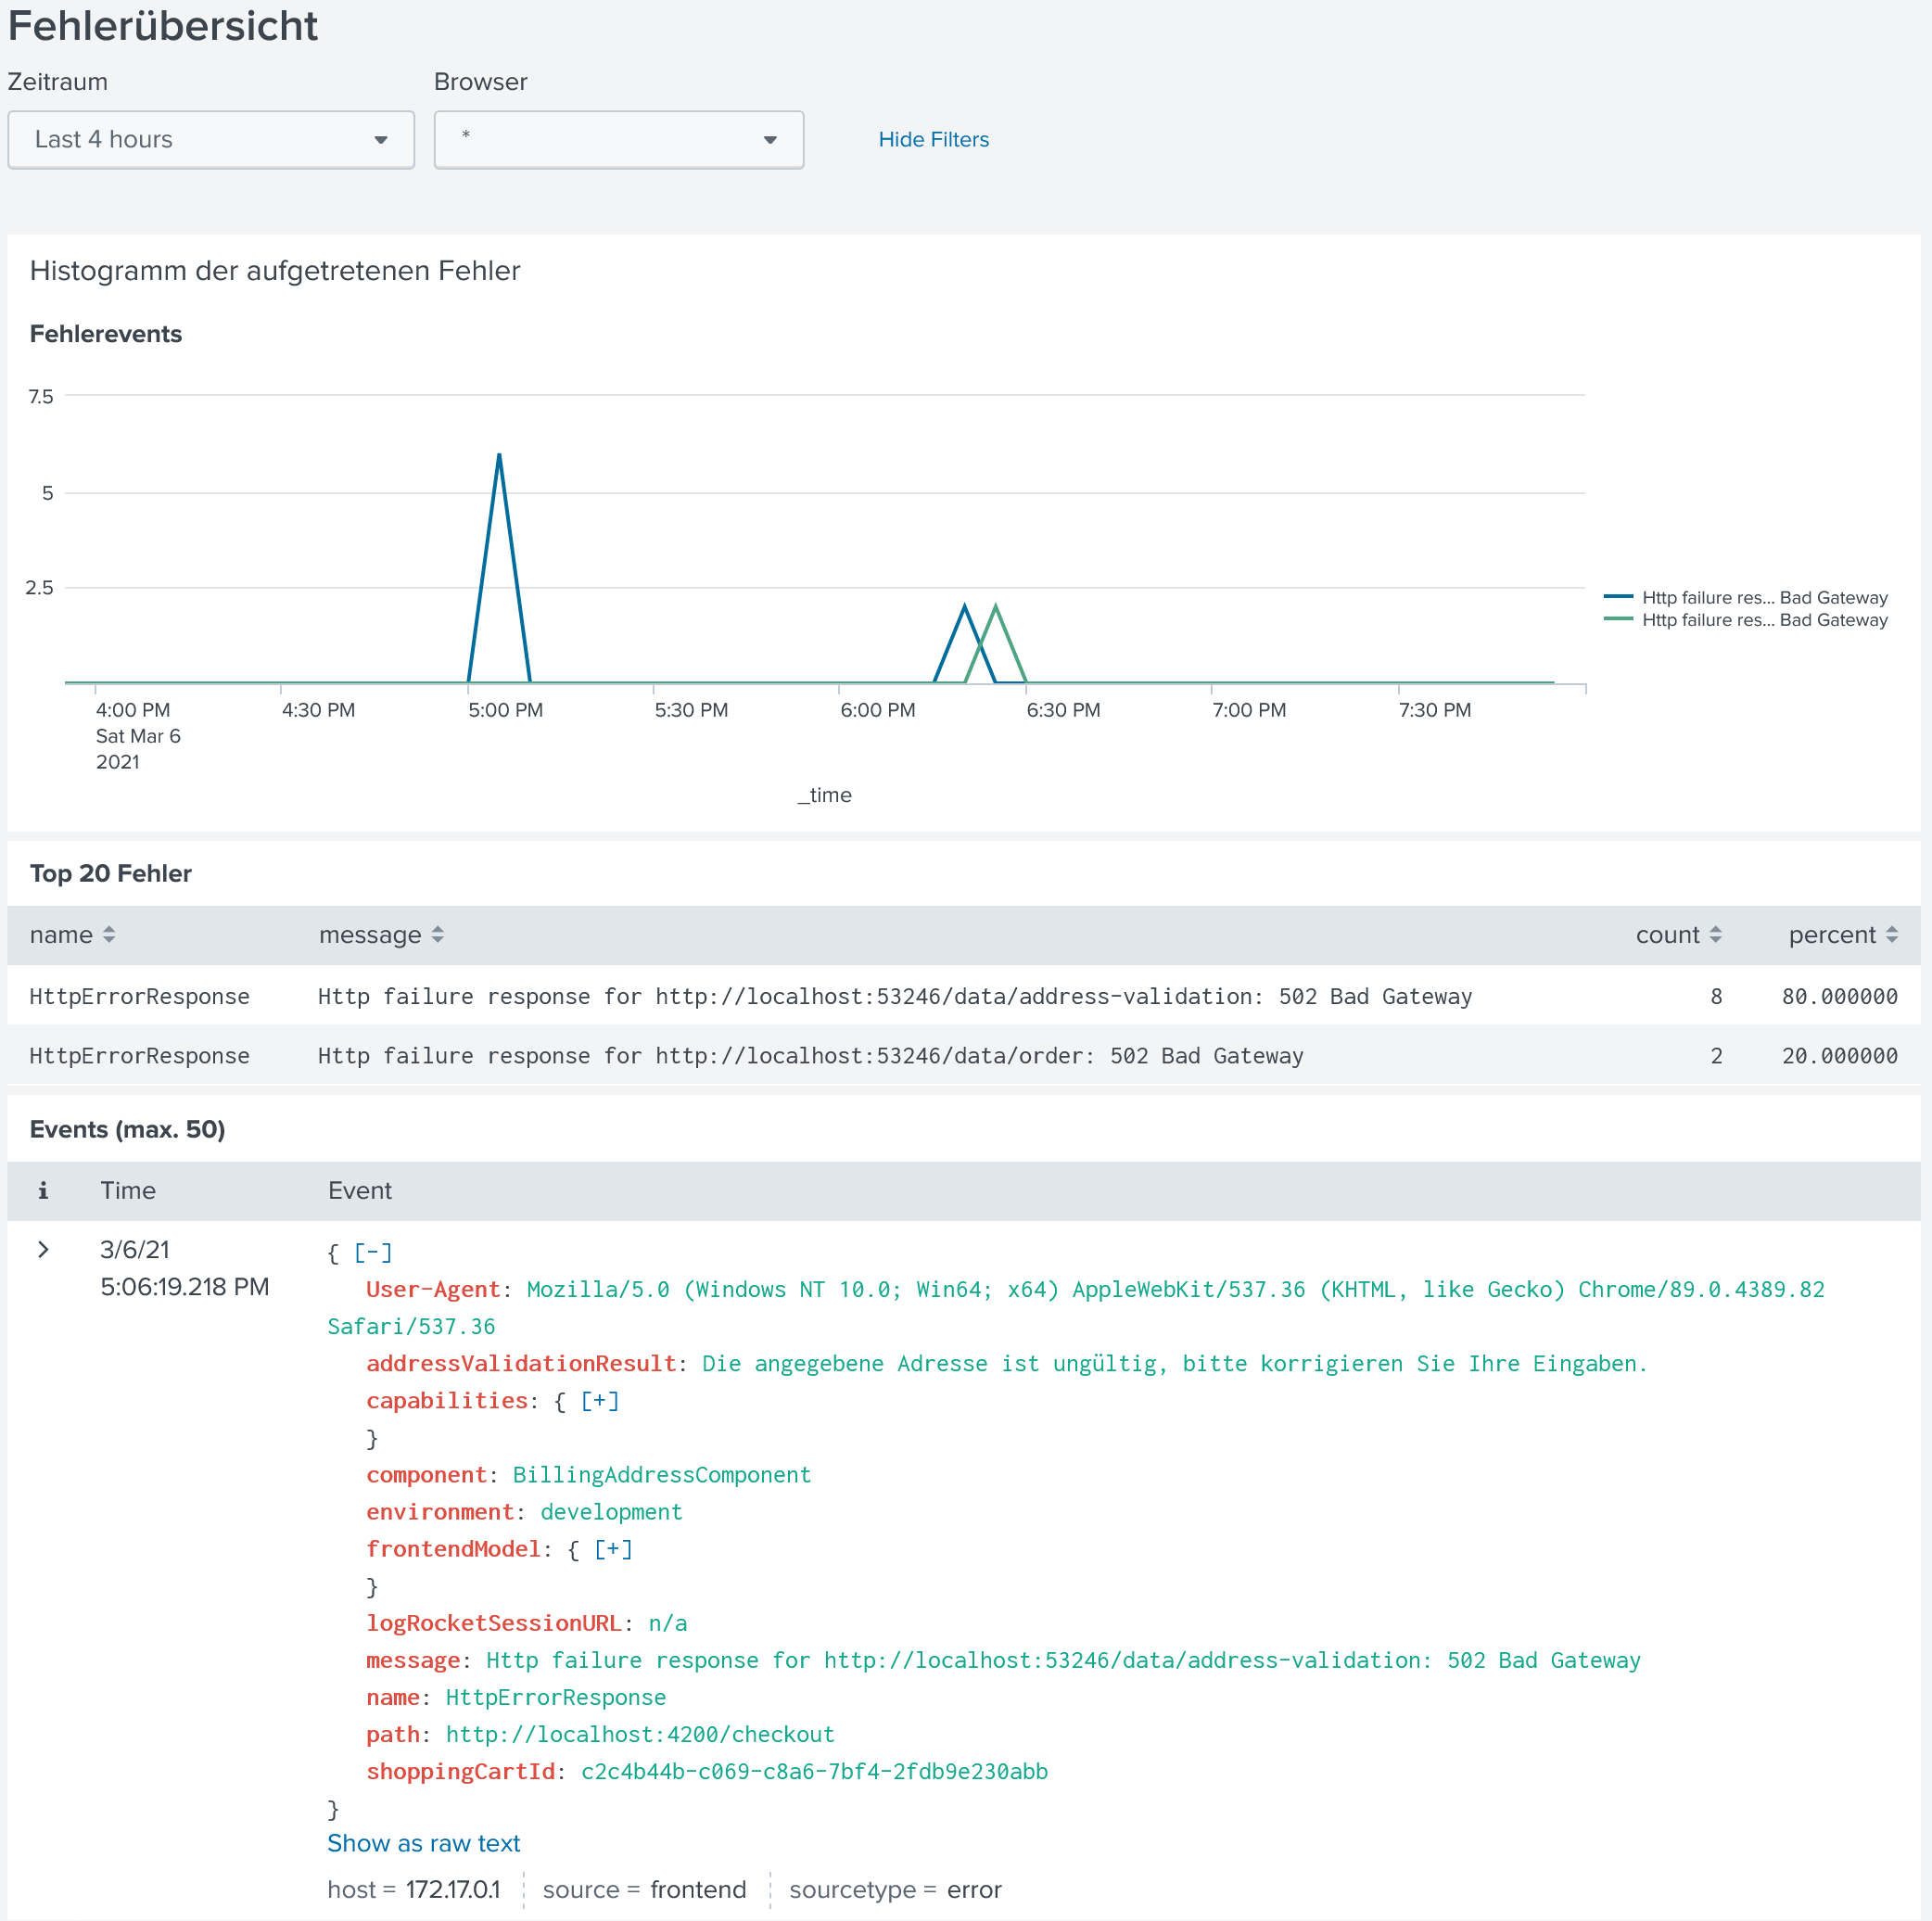
\includegraphics[width=1.00\linewidth]{img/99_postscript/splunk_error-dashboard.png}
	\caption{Fehlerübersicht in Splunk}
	\label{fig:splunk_error-dashboard}
\end{figure}

\subsection{Jaeger}
\label{sec:demo-jaeger}

In Jaeger lassen sich neben dem Trace-Gantt-Diagramm auch Traces miteinander vergleichen, sodass Unterschiede in den Aufrufen entdeckt werden können. In den Abbildungen \ref*{fig:jaeger_comparison-all} und \ref*{fig:jaeger_comparison-zoom} ist ein solcher Vergleich zu sehen. Hierbei werden Traces verglichen, die durch eine Anfrage von Warenkorb- und Übersetzungsdaten von Frontend aus resultiert sind. Dabei

 divergieren die beiden Traces in der Antwort vom Übersetzungsdienst, denn es wird bei einem Trace dort ein Fehler geworfen.

\begin{figure}[H]
	\centering
	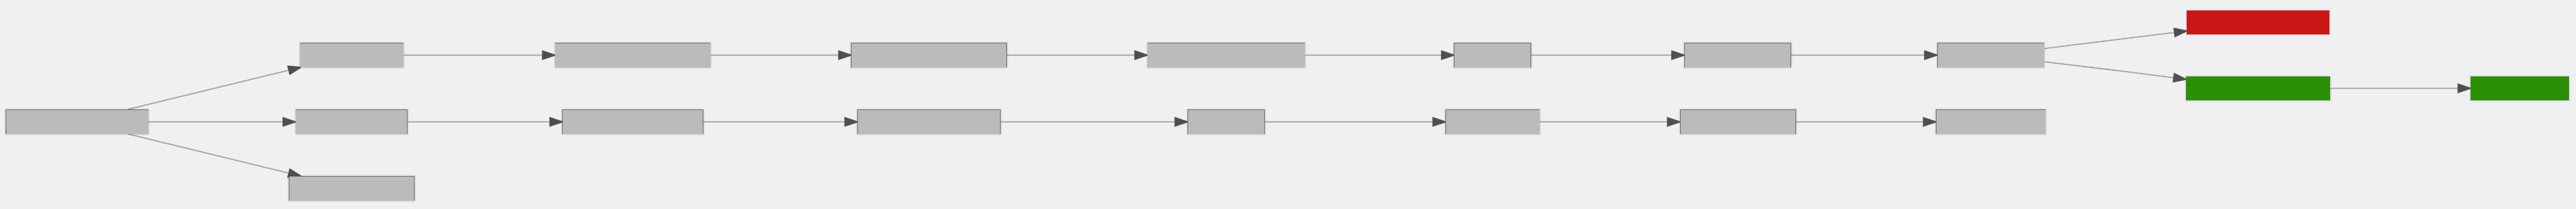
\includegraphics[width=1.00\linewidth]{img/99_postscript/jaeger_comparison-all.png}
	\caption{Tracevergleich in Jaeger}
	\label{fig:jaeger_comparison-all}
\end{figure}

\begin{figure}[H]
	\centering
	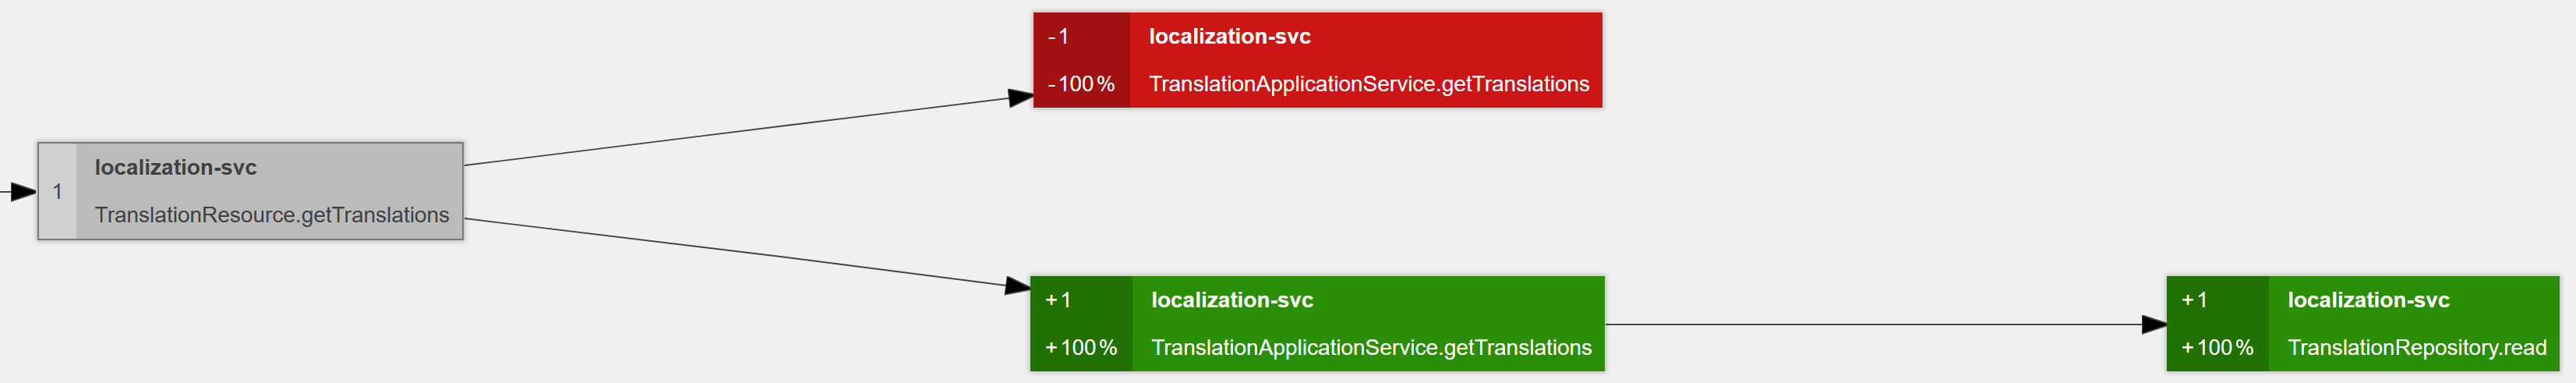
\includegraphics[width=1.00\linewidth]{img/99_postscript/jaeger_comparison-zoom.png}
	\caption{Tracevergleich in Jaeger (Zoom)}
	\label{fig:jaeger_comparison-zoom}
\end{figure}

Der von Jaeger automatisch erstellte Dienst-Abhängigkeits-Graph kann folgend in \autoref{fig:jaeger_service-dependency-graph} betrachtet werden.

\begin{figure}[H]
	\centering
	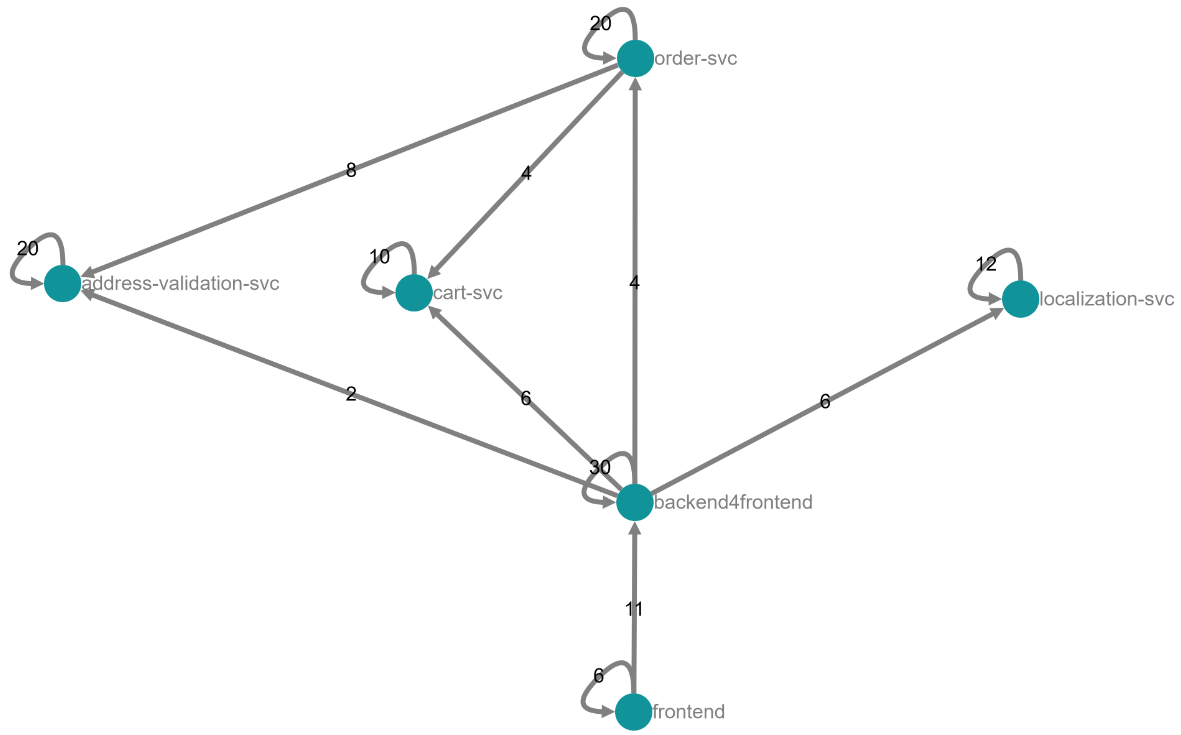
\includegraphics[width=0.7\linewidth]{img/99_postscript/jaeger_service-dependency-graph.png}
	\caption{Dienst-Abhängigkeits-Graph in Jaeger}
	\label{fig:jaeger_service-dependency-graph}
\end{figure}